%EM on the probabilistic model + algorithm
\section{Experiments}
In this section, we try to evaluate the performance of the two models on different datasets. We first present the experimental setup and the datasets used for the experiments. We then present the results obtained for the estimation algorithms on synthetic data and on real-life datasets. We finally try to discuss the results obtained and the relevance of the models. 

The goal of these experiments is to compare the two models but also to individually test their ability to cluster ordinal datasets and to check whether they are able to generalize to real-life datasets.

All of the experiments and table are reproducible using the provided code and datasets and the fixed seeds.

\subsection{Synthetic data}
\paragraph{Experimental setup.}
In this section, we propose to test the AECM algorithm for the BOS and the GOD model on synthetic data in order to check the ability of our proposed estimation methods to correctly estimate the parameters of the dataand to cluster the datasets. 

\paragraph{Runtimes.}
\label{sec:runtime}
The runtimes of the AECM algorithm implementation with exponential complexity from \citet{biernacki2016model} 
are compared to our implementation of the AECM algorithm with polynomial complexity. Figure~\ref{fig:runtime_epsilon}  compare both complexities for multiple runtimes for both univariate and multivariate AECM runs. The runtimes are reported with different number of categories in the dataset $m$. While the original implementation struggles to go further than $m=6$, our implementation can easily reach higher number of categories. The implementation ordinalClust \cite{selosse2021ordinalclust} is used for fair comparison and it is allowed to converge with a predefined $\epsilon$ parameter (internal to the authors package that we cannot modify). 
The worst case complexity of our implementation is plotted (with $300$ iterations without allowing it to terminate when converged) is plotted to highlight the time gains. The runtimes in the case where our implementation is stopped at convergence with an $\epsilon$ parameter, taken small enough for the comparison, are also plotted.
\begin{figure}[H]
    \centering
    \begin{subfigure}[b]{0.49\textwidth}
    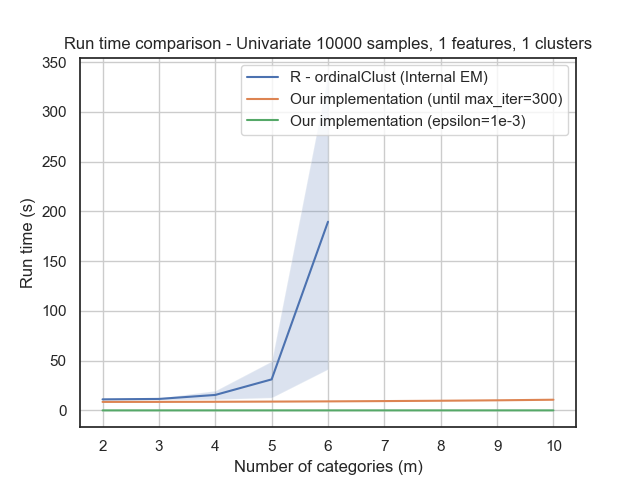
\includegraphics[width=1\textwidth]{python_figures/run_time_comparison_univariate_epsilon.png}
        \caption{Univariate case}
    \label{fig:runtime_univariate_epsilon}
    \end{subfigure}
    \hfill
    \begin{subfigure}[b]{0.49\textwidth}
    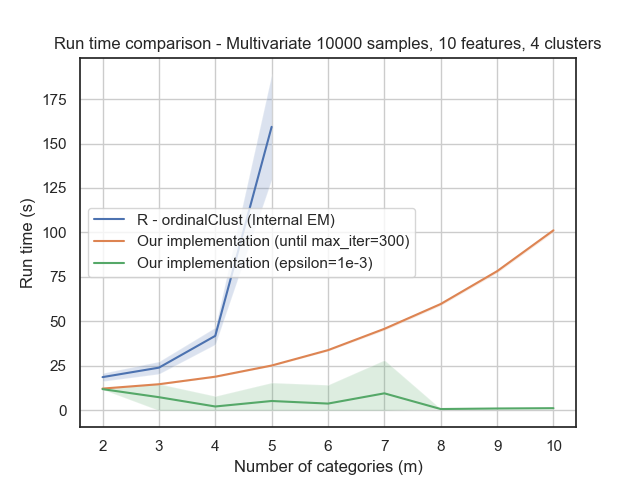
\includegraphics[width=1\textwidth]{python_figures/run_time_comparison_multivariate_epsilon.png}
        \caption{Multivariate case}
    \label{fig:runtime_multivariate_epsilon}
    \end{subfigure}
    \caption{Runtime comparison of the AECM algorithm for the BOS estimation on multivariate datasets as a function of the number of categories. For the ordinalClust package \cite{selosse2021ordinalclust}, nbSEM = 300, nbSEMburn = 200 and for our implementation, we run the model for $300$ iterations in the first curve (worst case) and set $\epsilon = 10^{-3}$ in the second curve. For every measurement, 10 datasets were generated and the average runtime is reported.}
    \label{fig:runtime_epsilon}
\end{figure}
For all the experiments, the runtimes are measured on the same machine for all the tests and over 10 runs.
% \ar{Plot with m going very high but just for our implementation?}

\paragraph{Evaluating the estimation error.}
We generate data from the BOS and the GOD model with different parameters and with both a random initialization of the parameters and an initialization of the parameters using the K-Means algorithm and then run the AECM algorithm on the generated data to estimate the parameters. We then compare the estimated parameters with the true parameters using the $L_1$ distance between the two vectors similarly to \cite{biernacki2016model}. We repeat this process multiple times for different parameters and average the results to obtain the metrics presented in Table~\ref{tab:results_bos} and Table~\ref{tab:results_god} in Appendix \ref{appendix:metrics_synth}. Runtimes are also measured on the same machine for all the algorithms to evaluate their efficiency.
The results show that on average, the parameter estimation is better with a random initialization than with a KMeans initialization. This is likely due to the fact that the KMeans initialization is not adapted to the ordinal nature of the data, and converges to local minima that are further from the ones from the initial distribution. Both the BOS and the GOD model parameters are being estimated with comparable accuracy.

\paragraph{Clustering performance.}
We also generate data with multiple clusters from different distributions and then run the AECM algorithm on the generated data to estimate the clusters. The goal of this experiment is to check the ability of the models to correctly cluster the data and to check whether the models are able to generalize to different distributions.
The distributions used are the BOS model, the GOD model and discretized blobs.
The following clustering algorithms are used for comparison: K-Means, Gaussian Mixture Models and the BOS and GOD models. The ARI score (section~\ref{sec:evaluation_method}) is used to measure the clustering performance. The results are presented in Table~\ref{tab:results_synth_clustering} of Appendix \ref{appendix:metrics_synth}.
% \ar{Need to add ordinal clustering algorithms that are different?}
% \ar{Discussion}
We notice that the data genearated from ordinal focus models like BOS or GOD are better classified by the BOS and GOD models than by the other models. At the same time, the BOS and GOD models are worse than KMeans and GMM on the blobs dataset. This is not surprising since the BOS and GOD models are specifically designed for ordinal data and it highlights the importance of using the right model for the right data.

\paragraph{Visualizing the clusters.}
In order to get a better idea of the differences between the clustering methods, t-SNE visualizations \citep{van2008visualizing} are plotted for different disitributions and clustering methods. The visualizations project the categorical datapoints in a continuous space and allow to check whether the estimated clusters are coherent with the true clusters. Since categorical data is used, it is more difficult to separate the clusters with smaller dimensionnal data and when the number of categories is small. Multiple datasets are generated with different parameters in order to highlight these differences. Moreover, as seen in the previous paragraph, it is also easier to cluster the data when the number of categories or features are high.
The results are presented in Figure~\ref{fig:tsne_comparative_analysis} of Appendix \ref{appendix:metrics_synth}. While the KMeans slgorithm identifies clusters that are well separated visually, 
it fails to identify the true clusters in the case of the BOS and GOD models, especially when the number of categories is small. Moreover, even in the case where even 4 features are used, we also notice that categorical clusters are not easy to separate as shown by the obtained ARI scores. This highlights the difficulty of clustering categorical data even with specific algorithms designed to do so for small number of features or small number of categories.
% \ar{Discussion}

\subsection{Real-life datasets}
\subsubsection{Datasets} One of the main goal of the experiments is to test the ability of the models to generalize to real-life datasets. We therefore propose to test the illustrated methods on real world datasets to check the usefulness of the models on different real-life situations. Since the algorithm is specifically designed for ordinal observations, the datasets need to be adapted for the task. One way to apply to obtain real-life datasets is to quantize continuous datasets of observations that can be categorized (e.g. movies, store products, species...) \citep{skubacz2000quantization}. Another interesting approach could be to test the models on tasks that they were not specifically designed for. This could allow seeing how they can generalize and whether they are applicable to a broader class of problems. We therefore propose to test the ability to cluster observations of binary features into different animal species.
\paragraph{Zoo Dataset.} The zoo dataset consists of multiple features describing $101$ different animals, with most of them being binary variables associated to a characteristic of the animal (hair, feathers, eggs, milk, \ldots) \citep{misc_zoo_111}. Every animal belongs to one of $6$ classes. 
\paragraph{Car Evaluation Dataset.} The car evaluation dataset consists of multiple features describing $1728$ different cars, with most of them being ordinal variables associated to a characteristic of the car (buying price, maintenance price, number of doors, \ldots) \citep{misc_car_evaluation_19}. Every car belongs to one of $4$ classes.
\paragraph{Hayes-Roth Dataset.} The Hayes-Roth dataset consists of multiple features describing $132$ different persons, with most of them being binary variables associated to a characteristic of the person (has a PhD, is married, is a professional, \ldots) \citep{misc_hayes_roth_44}. Every person belongs to one of $3$ classes.
\paragraph{Caesarian Dataset.} The Caesarian dataset is a dataset describing $80$ different patients with multiple features associated to the patient (age, delivery number, delivery time, blood pressure, \ldots) \citep{misc_caesarian_section_classification_dataset_472}. Every patient belongs to one of $2$ classes. \\ \\
The advantage of these datasets is that they are small enough to be able to compute the exact likelihood of the data given the model and the parameters. This allows to check whether the models are able to correctly fit the data.
\paragraph{Nursery School Dataset.} The Nursery School dataset is a dataset describing $12960$ different children with multiple features associated to the child (parents' occupation, family status, social conditions, \ldots) \citep{misc_nursery_76}. Every child belongs to one of $5$ classes. 
These classes are can also be interpreted as ordinal and represent the subjective quality of the nursery school that they attend. \\ \\

\subsubsection{Evaluation method.} \label{sec:evaluation_method}
For most of the real-life evaluation datasets, we will use classification tasks to check the ability to cluster with respect to pre-existing classes. This allows the evaluation framework to be easier to define. However, the results are very sensitive to the initial parameters used. In our evaluation, we keep the results for a unique seed, but it might be interesting to try different initialization scenarios in a real-life situation when trying to fit new data. 
Moreover, we are evaluating on the classification task, but the classes might not necessarily be the same as the clusters found (multiple classifications are possible in a dataset depending on the task).

In order to correctly associate the predicted clusters with the true clusters, we need to define a strategy that matches each predicted clusters with a true cluster number which will minimize a given criterion.
In order to do so, we propose two methods:
\begin{itemize}
    \item The first one consists in sorting the histograms of the predicted clusters and the true clusters and then matching the two sorted lists by assigning the predicted clusters to the true cluster in the same sorted order.
    
    This method is naive because it does not take into account the distribution of the real clusters according to the true labels for the matching.
    
\item The second method consists in solving the Assignment Problem \citep{kuhn1955hungarian} with the cost matrix being the distance between the histograms of the predicted clusters and the true clusters. This method takes into account the distribution of the real clusters according to the true labels for the matching. We can easily solve it using any Optimal Transport algorithm (or by defining the Linear Programming problem and solving it using an LP solver).
\end{itemize}
Figure \ref{fig:assignment_methods} of appendix \ref{appendix:metrics_real} shows that the optimal matching when considering the assignment matrix is a better choice in the case of the Zoo dataset for example and that the classes in the predicted distribution are assigned to the correct true class with respect to their proportions.


The evaluation metrics used to compare the different models are the F1-score, and the Accuracy score in the cases where the datasets are suited for classification and the Wasserstein distance and the Adjusted Rand Index (ARI).
\begin{itemize}
    \item The F1-score is the harmonic mean of the precision and the recall for classification problems.
    \item The Wasserstein distance is a measure of the distance between two probability distributions \citep{ramdas2017wasserstein}. 
        It measures the cost of transforming one distribution into the other using the optimal transport plan which in this case is the matching obtained as described above.
        \begin{equation}
            W(\hat{y}, y) = \min_{\gamma \in \Gamma(\hat{y}, y)} \sum_{i, j} \gamma_{i, j} \norm{i - j}
        ,\end{equation}
    where $\Gamma(\hat{y}, y)$ is the set of all possible matchings between the predicted clusters and the true clusters and $\gamma_{i, j}$ is the probability of matching the predicted cluster $i$ with the true cluster $j$ (i.e. it is the proportion of the samples in the predicted cluster $i$ that are in the true cluster $j$) for the matching.
\item The ARI is a measure of the similarity between two clusterings of the same dataset. It is a function that outputs a value between -0.5 and 1, where 1 means that the two clusterings are identical, 0 means that the two clusterings are independent (random) and -0.5 means that the two clusterings are as different as possible. The ARI is symmetric and therefore does not take into account the order of the clusters \citep{steinley2004properties}. 
    \begin{equation}
    \text{ARI}(\hat{y}, y) = \frac{\sum_{i, j} \binom{n_{i, j}}{2} - \left[\sum_i \binom{\hat{n}_i}{2} \sum_j \binom{n_j}{2}\right] / \binom{n}{2}}{\frac{1}{2} \left[\sum_i \binom{\hat{n}_i}{2} + \sum_j \binom{n_j}{2}\right] - \left[\sum_i \binom{\hat{n}_i}{2} \sum_j \binom{n_j}{2}\right] / \binom{n}{2}}
    ,\end{equation}
where $n_{i, j}$ is the number of samples that are in the predicted cluster $i$ and in the true cluster $j$, $\hat{n}_i$ is the number of samples in the predicted cluster $i$ and $n_j$ is the number of samples in the true cluster $j$.
\end{itemize}

\subsubsection{Experiments with real-life datasets}
To do so, we also use simple clustering algorithms to compare the performance of the BOS model on data that is adapted (ordinal) with algorithms that are not specifically designed for this kind of data such as K-Means \citep{macqueen1967some} and Gaussian Mixture Models \citep{reynolds2009gaussian}.
The results are presented in Table~\ref{tab:results_real} in the appendix \ref{appendix:metrics_real}. One interesting observation is that our implementation of the clustering methods scale well with the number of samples when comparaed to a Gaussian Mixture Model for example. 
During the experiments, the final results were very  sensitive to the initial parameters used, most notably the proportion of each clusters, and initializations are likely to get stuck on a local minimum because of the nature of AECM.
% We notice that although K-Means allows to significantly reduce the runtime of both the BOS and the GOD models estimations, it does not necessarily increase the clustering score and the classification score. The BOS model, because of its complexity, is also the longest to run but seems to be competitive with the other models on most datasets.
In order to get a better idea of the differences between the clustering methods, we also plot t-SNE visualizations \citep{van2008visualizing} for different datasets and the multiple models in Appendix~\ref{sec:appendix_assign}. The histogram and assignment matrix of the Zoo dataset are also provided in Appendix~\ref{sec:appendix_assign} in order to get a better understanding of the different assignments obtained in these settings for different models.

% \subsection{"experiment with a modification of the method"}





